\documentclass{beamer}
\usepackage[utf8]{inputenc}
\usepackage[T1]{fontenc}
\usepackage[norsk]{babel}
\usepackage{hyperref}
\usepackage{fancyvrb}


\usepackage{tikz}
\usepackage{amsmath}

\usetikzlibrary[topaths]
\usetikzlibrary{automata}
\usetikzlibrary{graphs}

\begin{document}

\begin{frame}
\begin{center}
\Huge{Tegnekurs i TikZ} \\
\vspace{10pt}
\Large{Veronika Heimsbakk}\\
veronahe@ulrik.uio.no
\end{center}
\end{frame}

%%% THE BASICS : LINJE%%%
\begin{frame}[fragile]
\frametitle{The Basics -- tegne ei linje}
\begin{center}
\begin{tikzpicture}
	\draw (0,0) -- (4,0);
\end{tikzpicture}
\end{center}

\vspace{20pt}

\begin{Verbatim}[fontsize=\small]
\begin{tikzpicture}
    \draw (0,0) -- (4,0);
\end{tikzpicture}
\end{Verbatim}

\end{frame}

%%% THE BASICS : KVADRAT%%%
\begin{frame}[fragile]
\frametitle{The Basics -- kvadrat}
\begin{center}
\begin{tikzpicture}
	\draw (0,0) rectangle (4,4);
\end{tikzpicture}
\end{center}

\vspace{20pt}
\begin{itemize}
\item
\begin{Verbatim}[fontsize=\small]
\draw (0,0) -- (4,0) -- (4,4) -- (0,4) -- (0,0);
\end{Verbatim}

\item
\begin{Verbatim}[fontsize=\small]
\draw (0,0) rectangle (4,4);
\end{Verbatim}
\end{itemize}
\end{frame}

%%% THE BASICS : SIRKEL%%%
\begin{frame}[fragile]
\frametitle{The Basics -- sirkel}
\begin{center}
\begin{tikzpicture}
	\draw (2,2) circle (1.5cm);
	\draw (6,2) ellipse (2cm and 1cm);
\end{tikzpicture}
\end{center}

\vspace{20pt}

\begin{itemize}
\item
\begin{Verbatim}[fontsize=\small]
\draw (2,2) circle (1.5cm);
\end{Verbatim}

\item
\begin{Verbatim}[fontsize=\small]
\draw (6,2) ellipse (2cm and 1cm);
\end{Verbatim}
\end{itemize}

\end{frame}

%%% THE BASICS : SIRKEL PYNT%%%
\begin{frame}[fragile]
\frametitle{The Basics -- pynte litt}
\begin{center}

\begin{tikzpicture}
	\draw[red, very thick, dashed] (2,2) circle (1.5cm);
	\draw[green, thick] (6,2) circle (1.5cm);
\end{tikzpicture}
\end{center}

\vspace{20pt}

\begin{itemize}
\item
\begin{Verbatim}[fontsize=\small]
\draw[red, very thick, dashed] (2,2) circle (1.5cm);
\end{Verbatim}

\item
\begin{Verbatim}[fontsize=\small]
\draw[green, thick] (6,2) circle (1.5cm);
\end{Verbatim}
\end{itemize}

\end{frame}

%%% THE BASICS : FARGER%%%
\begin{frame}[fragile]
\frametitle{The Basics -- fylle med farge}
\begin{center}
\begin{center}

\begin{tikzpicture}
	\fill[red] (0,0) rectangle (3,3);
\end{tikzpicture}
\end{center}
\end{center}

\vspace{20pt}

\begin{Verbatim}[fontsize=\small]
\fill[red] (0,0) rectangle (3,3);
\end{Verbatim}

\end{frame}

\begin{frame}[fragile]
\frametitle{The Basics -- fylle med farge og kant}
\begin{center}

\begin{tikzpicture}
	\filldraw[red!50, draw=black, very thick] (0,0) rectangle (3,3);
\end{tikzpicture}
\end{center}


\vspace{20pt}

\begin{Verbatim}[fontsize=\small]
\filldraw[red!50, draw=black, very thick] (0,0) rectangle (3,3);
\end{Verbatim}

\end{frame}

\begin{frame}[fragile]
\frametitle{The Basics -- fylle med gradient}
\begin{center}

\begin{tikzpicture}
	\shade[left color=black, right color=red] (0,0) rectangle (3,3);
\end{tikzpicture}
\end{center}

\vspace{20pt}

\begin{Verbatim}[fontsize=\small]
\shade[left color=black, right color=red] (0,0) rectangle (3,3);
\end{Verbatim}

\end{frame}


%%% KOORDINATSYSTEM: RUTENETT%%%
\begin{frame}[fragile]
\frametitle{Rutenett med akser}
\begin{center}
\scalebox{0.5}{%
\begin{minipage}{\textwidth}
\begin{tikzpicture}
    \draw[step=1cm,gray,very thin] (-1.9,-1.9) grid (5.9,5.9);
\end{tikzpicture}
\end{minipage}%
}  
\end{center}

\vspace{20pt}

\begin{Verbatim}[fontsize=\small]
\draw[step=1cm,gray,very thin] (-1.9,-1.9) grid (5.9,5.9);
\end{Verbatim}

\end{frame}

%%% KOORDINATSYSTEM: AKSER%%%
\begin{frame}[fragile]
\frametitle{Rutenett med akser}
\begin{center}
\scalebox{0.5}{%
\begin{minipage}{\textwidth}
\begin{center}
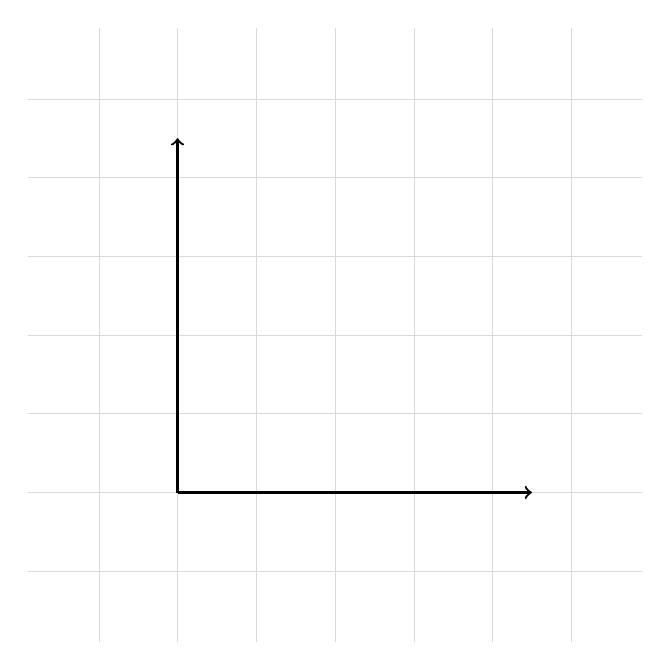
\begin{tikzpicture}
    \draw[step=1cm,gray!30,very thin] (-1.9,-1.9) grid (5.9,5.9);
    \draw[thick, ->] (0,0) -- (4.5,0);
    \draw[thick, ->] (0,0) -- (0,4.5);
\end{tikzpicture}
\end{center}
\end{minipage}%
}  
\end{center}

\vspace{20pt}

\begin{Verbatim}[fontsize=\small]
\draw[step=1cm,gray!30,very thin] (-1.9,-1.9) grid (5.9,5.9);
\draw[thick, ->] (0,0) -- (4.5,0);
\draw[thick, ->] (0,0) -- (0,4.5);
\end{Verbatim}

\end{frame}

%%% KOORDINATSYSTEM: LABEL%%%
\begin{frame}[fragile]
\frametitle{Rutenett med akser}
\begin{center}
\scalebox{0.5}{%
\begin{minipage}{\textwidth}
\begin{center}

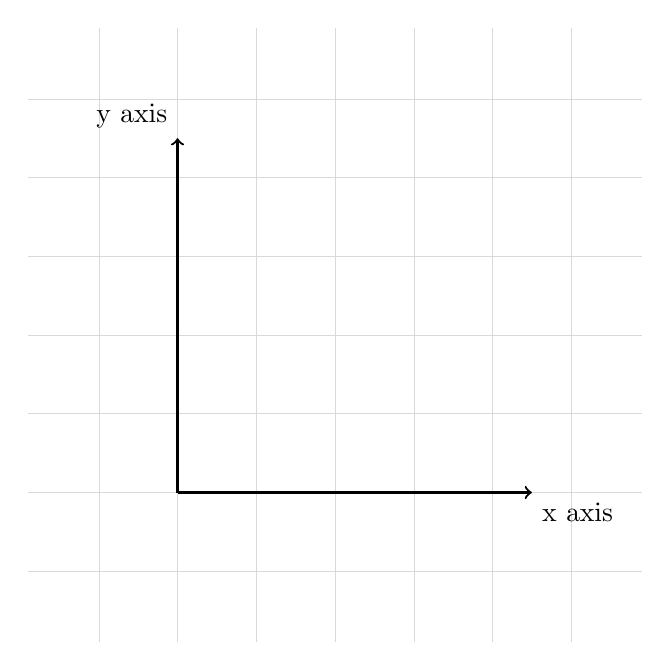
\begin{tikzpicture}
    \draw[step=1cm,gray!30,very thin] (-1.9,-1.9) grid (5.9,5.9);
    \draw[thick, ->] (0,0) -- (4.5,0) node[anchor=north west] {x axis};
    \draw[thick, ->] (0,0) -- (0,4.5) node[anchor=south east] {y axis};
\end{tikzpicture}
\end{center}

\end{minipage}%
}  
\end{center}

\vspace{20pt}


\begin{Verbatim}[fontsize=\footnotesize]
\draw[thick, ->] (0,0) -- (4.5,0) node[anchor=north west] {x axis};
\draw[thick, ->] (0,0) -- (0,4.5) node[anchor=south east] {y axis};
\end{Verbatim}

\end{frame}

%%% KOORDINATSYSTEM: LABEL OG TALL%%%
\begin{frame}[fragile]
\frametitle{Rutenett med akser}
\begin{center}
\scalebox{0.5}{%
\begin{minipage}{\textwidth}
\begin{center}
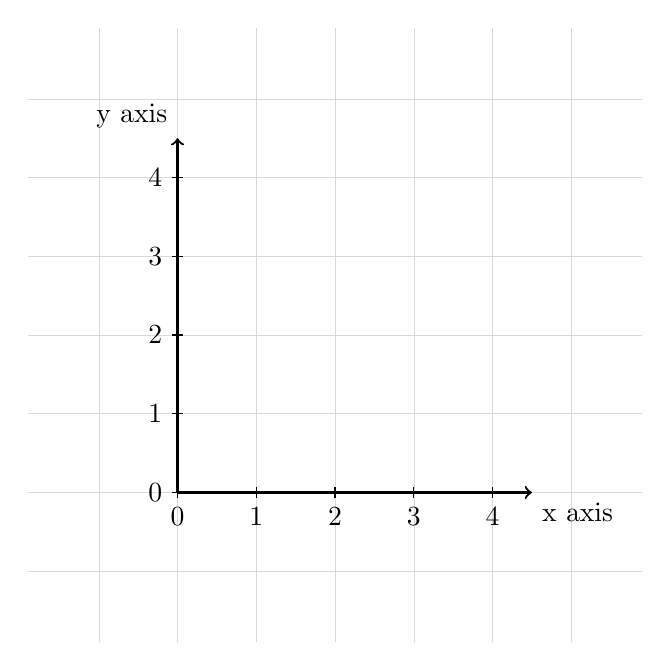
\begin{tikzpicture}
    \draw[step=1cm,gray!30,very thin] (-1.9,-1.9) grid (5.9,5.9);
    \draw[thick, ->] (0,0) -- (4.5,0) node[anchor=north west] {x axis};
    \draw[thick, ->] (0,0) -- (0,4.5) node[anchor=south east] {y axis};

    \foreach \x in {0,1,2,3,4}
	\draw (\x cm, 2pt) -- (\x cm, -2pt) node[anchor=north] {$\x$};
    \foreach \y in {0,1,2,3,4}
	\draw (2pt, \y cm) -- (-2pt, \y cm) node[anchor=east] {$\y$};
\end{tikzpicture}
\end{center}

\end{minipage}%
}  
\end{center}

\vspace{20pt}

\begin{Verbatim}[fontsize=\footnotesize]
\foreach \x in {0,1,2,3,4}
   \draw (\x cm, 2pt) -- (\x cm, -2pt) node[anchor=north] {$\x$};
\foreach \y in {0,1,2,3,4}
   \draw (2pt, \y cm) -- (-2pt, \y cm) node[anchor=east]  {$\y$};
\end{Verbatim}

\end{frame}

%%% TRÆR: ILLUSTRASJON %%%
\begin{frame}[fragile]
\frametitle{Trær}

\begin{center}
\begin{tikzpicture}[every node/.style={},level 2/.style={sibling distance=20mm},
				   level 3/.style={sibling distance=10mm}, level distance=30pt]
\node {S}
	child { node{A} 
		child { node {A} 
			child { node {(} }
			child { node {)} }
		}
		child { node {A} 
			child { node {(} }
			child { node {A} 
				child { node {(} }
				child { node {)} }
			}
			child { node {)} }
		}
	};
\end{tikzpicture}
\end{center}

\end{frame}

\begin{frame}[fragile]
\frametitle{Trær -- bygge et tre}

Rot-noden:
\begin{center}
\begin{tikzpicture}[every node/.style={},level 2/.style={sibling distance=20mm},
				   level 3/.style={sibling distance=10mm}, level distance=30pt]
\node {1};
\end{tikzpicture}
\end{center}

\begin{Verbatim}[fontsize=\small]
\node {1};
\end{Verbatim}

Bygger videre:

\begin{center}
\begin{tikzpicture}[every node/.style={},level 1/.style={sibling distance=10mm},
				   level 3/.style={sibling distance=10mm}, level distance=25pt]
\node {1}
	child {node {2}}
	child {node {3}
		child {node {4} }
		child {node {5} }
	}
;
\end{tikzpicture}
\end{center}

\begin{Verbatim}[fontsize=\small]
\node {1}
    child { node {2} }
    child { node {3} 
        child { node {4} }
        child { node {5} }
    }
;
\end{Verbatim}


\end{frame}

%%% TRÆR: KODEN %%%
\begin{frame}[fragile]
\frametitle{Trær}

\begin{Verbatim}[fontsize=\footnotesize, frame=single]
\begin{tikzpicture}[every node/.style={},
                    level 2/.style={sibling distance=20mm},
                    level 3/.style={sibling distance=10mm}, 
                    level distance=30pt]
\node {S}
    child { node{A} 
        child { node {A} 
            child { node {(} }
            child { node {)} }
        }
        child { node {A} 
            child { node {(} }
            child { node {A} 
                child { node {(} }
                child { node {)} }
            }
            child { node {)} }
        }
    }
;
\end{tikzpicture}
\end{Verbatim}

\end{frame}

%%% TRÆR: RØD-SVART %%%
\begin{frame}[fragile]
\frametitle{Rød-svarte trær}


\tikzset{
	treenode/.style = {align=center, inner sep=0pt},
	% Sorte noder
  	node_black/.style = {treenode, circle, white, font=\bfseries, draw=black,fill=black, text width=0.8cm},
	% Røde noder
  	node_red/.style = {treenode, circle, red, draw=red, text width=0.8cm, very thick},
	% Null-pekere
  	node_null/.style = {treenode, rectangle, draw=black, minimum width=0.3cm, minimum height=0.3cm}
}

\begin{center}
% Skal tegne med piler (->), og setter level/.style={opt.} %
\begin{tikzpicture}[->,level/.style={sibling distance = 2cm, level distance = 1.5cm}] 
\node [node_black] {38}
    	child{ node [node_red] {19} 
		child{node [node_black] {12}
			child{node [node_red] {8}}
			child{node [node_null] {}}
		}
		child{node [node_black] {31}}
	}
    	child{ node [node_black] {41} }
; 
\end{tikzpicture}
\end{center}

\end{frame}

%%% TRÆR: RØD-SVART STIL KODE %%%
\begin{frame}[fragile]
\frametitle{Trær}

\begin{Verbatim}[fontsize=\footnotesize, frame=single]
\tikzset{
   treenode/.style = {align=center, inner sep=0pt},
	
   % Sorte noder
   node_black/.style = {treenode, circle, white, 
		                  	     font=\bfseries, draw=black,
			                        fill=black, text width=0.8cm},
   % Røde noder
   node_red/.style = {treenode, circle, red, draw=red, 
	                      text width=0.8cm, very thick},
   % Null-pekere
   node_null/.style = {treenode, rectangle, draw=black, 
		                       minimum width=0.3cm, 
                       minimum height=0.3cm}
}
\end{Verbatim}

\end{frame}


%%% TRÆR: RØD-SVART KODE %%%
\begin{frame}[fragile]
\frametitle{Trær}

\begin{Verbatim}[fontsize=\footnotesize, frame=single]
\begin{tikzpicture}[->,level/.style={ sibling distance = 2cm, 
                    level distance = 1.5cm }] 

\node [node_black] {38}
    child {node [node_red] {19} 
        child {node [node_black] {12}
             child {node [node_red] {8} }
             child {node [node_null] {} }
        }
        child {node [node_black] {31} }
    }
    child { node [node_black] {41} }
; 
\end{tikzpicture}
\end{Verbatim}

\end{frame}


%%% GRAFER %%%
\begin{frame}[fragile]
\frametitle{Grafer}

\begin{center}
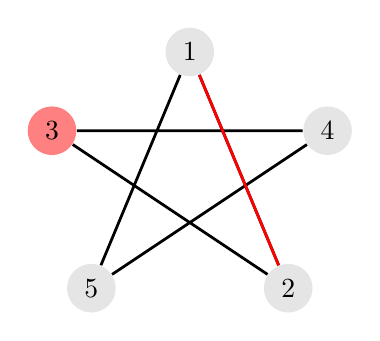
\begin{tikzpicture}[scale=5]
	 \tikzstyle{vertex}=[circle,fill=black!10]
	 \tikzstyle{selected vertex} = [vertex, fill=red!50]

	 \tikzstyle{selected edge} = [draw,line width=1pt,-,red!100]
	 \tikzstyle{edge} = [-,black,line width=1pt]

	 \node[vertex] (v1) at (1.25,1.7) 			{1};
	 \node[vertex] (v2) at (1.5,1.1) 				{2};
	 \node[selected vertex] (v3) at (0.9,1.5) 		{3};
	 \node[vertex] (v4) at (1.6,1.5) 				{4};
	 \node[vertex] (v5) at (1,1.1) 				{5};

	\draw[edge] (v1)  -- (v2) -- (v3) -- (v4) -- (v5) -- (v1); 
	\draw[selected edge] (v1) -- (v2);
\end{tikzpicture}
\end{center}

\begin{itemize}
\item
Noder (\texttt{vertex}) 
\item
Markerte noder (\texttt{selected vertex})
\item
Kanter (\texttt{edge})
\item
Markerte kanter (\texttt{selected edge})
\end{itemize}

\end{frame}


%%% GRAFER : NODER %%%
\begin{frame}[fragile]
\frametitle{Grafer -- noder}

\begin{center}

\begin{tikzpicture}[scale=5]
	 \tikzstyle{vertex}=[circle,fill=black!10]
	 \tikzstyle{selected vertex} = [vertex, fill=red!50]

	 \tikzstyle{selected edge} = [draw,line width=1pt,-,red!100]
	 \tikzstyle{edge} = [-,black,line width=1pt]

	 \node[vertex] (v1) at (0,0) {1};
	\node[selected vertex] (v2) at (0.5,0) {2};
\end{tikzpicture}
\end{center}

\begin{Verbatim}[fontsize=\small]
\tikzstyle{vertex} = [circle,fill=black!10]
\tikzstyle{selected vertex} = [vertex, fill=red!50]

% Tegne nodene
\node[vertex] (v1) at (0,0) {1};
\node[selected vertex] (v2) at (0.5,0) {2};
\end{Verbatim}

\end{frame}

%%% GRAFER : KANTER %%%
\begin{frame}[fragile]
\frametitle{Grafer -- kanter}

\begin{center}
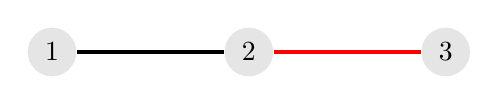
\begin{tikzpicture}[scale=5]
	 \tikzstyle{vertex}=[circle,fill=black!10]
	 \tikzstyle{selected vertex} = [vertex, fill=red!50]

	 \tikzstyle{selected edge} = [draw,line width=1.5pt,-,red!100]
	 \tikzstyle{edge} = [-,black,line width=1.5pt]

	 \node[vertex] (v1) at (0,0) {1};
	\node[vertex] (v2) at (0.5,0) {2};
	\node[vertex] (v3) at (1,0) {3};

	\draw[edge] (v1) -- (v2);
	\draw[selected edge] (v2) -- (v3);
\end{tikzpicture}
\end{center}

\begin{Verbatim}[fontsize=\small]
\tikzstyle{selected edge} = [draw,line width=1pt,-,red!100]
\tikzstyle{edge} = [-,black,line width=1pt]

% Tegne nodene
\node[vertex] (v1) at (0,0)   {1};
\node[vertex] (v2) at (0.5,0) {2};
\node[vertex] (v3) at (1,0)   {3};

% Tegne kantene
\draw[edge] (v1) -- (v2);
\draw[selected edge] (v2) -- (v3);
\end{Verbatim}

\end{frame}

%%% GRAFER : KANTER %%%
\begin{frame}[fragile]
\frametitle{Grafer -- kanter}


\begin{Verbatim}[fontsize=\footnotesize, frame=single]
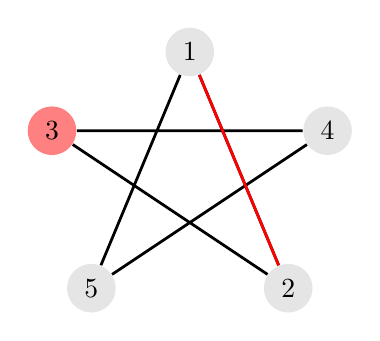
\begin{tikzpicture}[scale=5]
    \tikzstyle{vertex}         = [circle,fill=black!10]
    \tikzstyle{selected vertex}= [vertex, fill=red!50]

    \tikzstyle{selected edge}  = [draw,line width=1pt,-,red!100]
    \tikzstyle{edge}           = [-,black,line width=1pt]

    \node[vertex]          (v1) at (1.25,1.7) {1};
    \node[vertex]          (v2) at (1.5,1.1)  {2};
    \node[selected vertex] (v3) at (0.9,1.5)  {3};
    \node[vertex]          (v4) at (1.6,1.5)  {4};
    \node[vertex]          (v5) at (1,1.1)    {5};

    \draw[edge]          (v1)--(v2)--(v3)--(v4)--(v5)--(v1); 
    \draw[selected edge] (v1)--(v2);
\end{tikzpicture}
\end{Verbatim}

\end{frame}


%%% AUTOMATER %%%
\begin{frame}[fragile]
\frametitle{Automater}


\begin{center}
\scalebox{0.8}{%
\begin{minipage}{\textwidth}
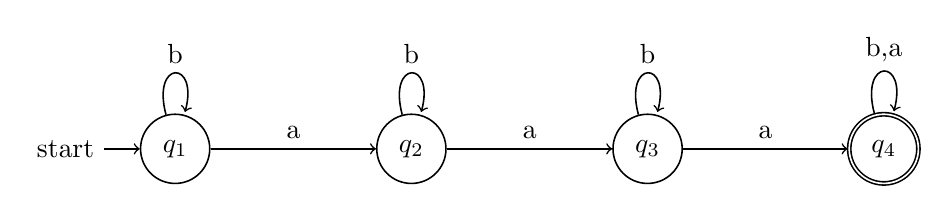
\begin{tikzpicture}[->,auto,node distance=3cm,line width=0.2mm]
  \node[initial,state] 			(A)		 	         {$q_1$};
  \node[state]         			(B) [right of=A] 	{$q_2$};
  \node[state]				(C) [right of=B] 	{$q_3$};
  \node[state,accepting]		(D) [right of=C] 	{$q_4$};

  \path 	(A) edge [loop above] node 			{b} 		(A)
			edge node 						{a} 		(B)
        		(B) edge [loop above] node 			{b} 		(B)
			edge node 						{a} 		(C)
		(C) edge [loop above] node 			{b}		(C)
			edge node 						{a} 		(D)
		(D) edge [loop above] node 			{b,a}	(D);
\end{tikzpicture}
\end{minipage}%
}  
\end{center}

Må inkludere \texttt{\textbackslash usetikzlibrary\{automata\}}.

\end{frame}

%%% AUTOMATER: KODE %%%
\begin{frame}[fragile]
\frametitle{Automater}


\begin{Verbatim}[fontsize=\footnotesize, frame=single]
\begin{tikzpicture}[->,auto,node distance=3cm,line width=0.2mm]
  \node[initial,state   (A) 	          	    {$q_1$};
  \node[state]          (B) [right of=A]    {$q_2$};
  \node[state]	         (C) [right of=B]    {$q_3$};
  \node[state,accepting](D) [right of=C]    {$q_4$};

  \path (A) edge [loop above] node 	 {b}   (A)
	    edge node      			                 {a}   (B)
        (B) edge [loop above] node 	 {b}   (B)
	    edge node   	                    {a}   (C)
        (C) edge [loop above] node	  {b}   (C)
	    edge node 	    	                 {a}   (D)
        (D) edge [loop above] node 	 {b,a} (D);
\end{tikzpicture}
\end{Verbatim}

\end{frame}


\end{document}